% Rapport de projet : Deep Learning for Spare Parts Management
% Compilation : xelatex (deux passes). Les graphiques lisent les fichiers de data/,
% produits par scripts/export_report_data.py.

\documentclass[11pt,a4paper]{article}

\usepackage{amsmath}
\usepackage{fontspec}
\usepackage{unicode-math}
\usepackage[french]{babel}
\frenchsetup{StandardLists=true}

\setmainfont{Palatino Linotype}
\setsansfont{Segoe UI}[BoldFont={Segoe UI Semibold}]
\newfontfamily\affiche{Segoe UI Light}
\setmathfont{Cambria Math}

\usepackage[top=2.7cm,bottom=2.6cm,left=2.5cm,right=2.5cm,headheight=15pt,headsep=0.8cm,footskip=1.2cm]{geometry}
\usepackage{xcolor}
\definecolor{primaire}{HTML}{1F3B57}
\definecolor{accent}{HTML}{C0602E}
\definecolor{fond}{HTML}{EEF2F6}
\definecolor{gris}{HTML}{6F7C89}

\usepackage{microtype}
\usepackage{setspace}
\setstretch{1.12}
\setlength{\parindent}{0pt}
\setlength{\parskip}{0.55em}

\usepackage{titlesec}
\usepackage{titletoc}
\usepackage{fancyhdr}
\usepackage{lastpage}
\usepackage{booktabs,tabularx,array,makecell,ragged2e,ltablex}
\keepXColumns
\setlength{\LTpre}{0.4em}
\setlength{\LTpost}{0.9em}
\usepackage{enumitem}
\usepackage{float}
\usepackage{needspace}
\usepackage{caption}
\usepackage{graphicx}
\usepackage{tikz}
\usetikzlibrary{arrows.meta,positioning,calc}
\usepackage{pgfplots}
\usepackage{pgfplotstable}
\pgfplotsset{compat=1.18}
\usepackage{hyperref}
\hypersetup{colorlinks=true,linkcolor=primaire,citecolor=accent,urlcolor=accent,
  pdftitle={Rapport de projet, Deep Learning for Spare Parts Management},
  pdfauthor={Adam Elmadani}}
\urlstyle{same}

\titleformat{\section}{\sffamily\fontsize{17}{21}\selectfont\color{primaire}}
  {\textcolor{accent}{\thesection}}{0.7em}{}[\nopagebreak\vspace{-0.3em}\nopagebreak{\color{primaire!18}\titlerule[0.8pt]}]
\titlespacing*{\section}{0pt}{2.0em}{1.1em}
\titleformat{\subsection}{\sffamily\bfseries\fontsize{12.5}{15}\selectfont\color{primaire}}
  {\thesubsection}{0.7em}{}
\titlespacing*{\subsection}{0pt}{1.4em}{0.4em}
\newcommand{\intertitre}[1]{\par\vspace{0.3em}{\sffamily\bfseries\color{primaire}#1}\par\vspace{-0.2em}}

\titlecontents{section}[0pt]{\addvspace{7pt}\sffamily\bfseries\color{primaire}}
  {\contentslabel{1.7em}}{}{\hfill\contentspage}
\titlecontents{subsection}[1.7em]{\addvspace{1pt}\small}
  {\contentslabel{2.4em}}{}{\titlerule*[0.7pc]{.}\contentspage}

\pagestyle{fancy}
\fancyhf{}
\fancyhead[R]{\sffamily\footnotesize\color{gris}\nouppercase{\leftmark}}
\fancyfoot[L]{\sffamily\footnotesize\color{gris}ENSAM, semestre 9}
\fancyfoot[R]{\sffamily\footnotesize\color{gris}\thepage\ / \pageref*{LastPage}}
\renewcommand{\headrulewidth}{0pt}
\renewcommand{\sectionmark}[1]{\markboth{\thesection\quad #1}{}}

\setlist{itemsep=0.2em,topsep=0.3em,leftmargin=1.4em}
\setlist[itemize,1]{label={\textcolor{accent}{\small\textbullet}}}

\renewcommand{\arraystretch}{1.28}
\newcolumntype{L}{>{\RaggedRight\arraybackslash}X}
\newcolumntype{P}[1]{>{\RaggedRight\arraybackslash}p{#1}}
\newcolumntype{R}{>{\RaggedLeft\arraybackslash}X}
\newcommand{\hd}[1]{\leavevmode{\sffamily\bfseries\color{primaire}#1}}
% Lignes de tableau générées par scripts/export_report_data.py. La primitive \@@input, à la
% différence de \input, ne laisse rien derrière elle qui ouvrirait une cellule avant \bottomrule.
\makeatletter
\newcommand{\lignes}[1]{\@@input #1 }
\makeatother
\setlength{\heavyrulewidth}{0.9pt}
\setlength{\lightrulewidth}{0.4pt}
\captionsetup{font=small,labelfont={sf,bf,color=primaire},labelsep=period,
  justification=raggedright,singlelinecheck=false,skip=6pt}
\captionsetup[table]{position=top}
\addto\captionsfrench{%
  \renewcommand{\tablename}{Tableau}%
  \renewcommand{\contentsname}{Sommaire}%
  \renewcommand{\refname}{Références}}

\pgfplotsset{
  rapport/.style={
    width=\linewidth, height=6.2cm,
    axis lines*=left, axis line style={gris!60},
    tick style={draw=none},
    ticklabel style={font=\sffamily\footnotesize, text=gris!90!black},
    label style={font=\sffamily\footnotesize, text=gris!90!black},
    legend style={font=\sffamily\footnotesize, draw=none, fill=none},
    ymajorgrids, grid style={gris!15},
  },
}

\begin{document}

% ---------------------------------------------------------------- Page de garde
\begin{titlepage}
\begin{tikzpicture}[remember picture,overlay]
  \fill[primaire] (current page.north west) rectangle ([xshift=1.3cm]current page.south west);
  \fill[accent] ([xshift=1.3cm]current page.north west) rectangle ([xshift=1.42cm]current page.south west);
\end{tikzpicture}
\sffamily
\vspace*{0.4cm}
{\small\color{gris}\addfontfeatures{LetterSpace=6}ÉCOLE NATIONALE SUPÉRIEURE D'ARTS ET MÉTIERS}\par
\vspace{3pt}
{\small\color{gris}Semestre 9 \quad·\quad Année universitaire 2026-2027}\par
\vspace{6.2cm}
{\color{accent}\rule{2.4cm}{2.5pt}}\par
\vspace{0.7cm}
{\affiche\fontsize{36}{42}\selectfont\color{primaire}Rapport de projet}\par
\vspace{0.55cm}
{\fontsize{17}{21}\selectfont\color{primaire!80}Deep Learning for Spare Parts Management}\par
\vspace{0.45cm}
\parbox{13cm}{\rmfamily\large\itshape\color{gris!80!black}Pilotage conjoint de la maintenance et du stock de pièces de rechange d'une flotte de machines industrielles}\par
\vfill
\renewcommand{\arraystretch}{1.35}
\begin{tabular}{@{}l@{\hspace{1.4cm}}l@{}}
\textcolor{gris}{Réalisé par} & Adam Elmadani \\
\textcolor{gris}{Encadré par} & Pr. Aziza Belmaati \\
 & Pr. Oumaima Bounou \\
\textcolor{gris}{Version} & 1.0, octobre 2026 \\
\end{tabular}
\vspace*{0.3cm}
\end{titlepage}

{\sffamily\fontsize{14}{17}\selectfont\color{primaire}Résumé}\par
\vspace{0.3em}
Ce projet étudie le pilotage conjoint de la maintenance et du stock de pièces de rechange d'une flotte de 100 machines réparties en deux familles, l'une vieillissant à l'usage, l'autre au calendrier. Un simulateur à événements discrets reproduit pannes, maintenances, approvisionnements, défauts de fabrication et télémétrie ; calibré sur le jeu Microsoft Azure Predictive Maintenance, il retrouve le nombre de pannes de chaque composant sur l'année 2015 à moins de 10~\% près. Des réseaux de survie récurrents et convolutifs estiment le risque de panne de chaque composant à partir de 48 heures de signaux ; ils dépassent LightGBM sur données simulées et, à 7 jours, sur données réelles. Une politique prédictive fondée sur ces réseaux réduit le coût annuel de 2,1~\% par rapport à une politique à seuils fixes optimisés, écart significatif sur 30 années simulées, mais une maintenance conditionnelle simple fait mieux encore, avec 9,6~\% d'économie. Les agents d'apprentissage par renforcement profond (PPO avec masquage d'actions, DQN, Branching Dueling Q-Network) n'atteignent pas la politique à seuils optimisés : le meilleur, qui règle chaque jour les seuils de maintenance et de stock, s'en approche à 1,1~\% près, tandis que les agents qui décident machine par machine restent loin derrière. Un modèle de substitution ($R^2$ de 0,98 sur le coût) permet l'analyse de sensibilité de Sobol, et une application web restitue l'ensemble.


\vspace{1cm}
\tableofcontents
\newpage

% ================================================================ 1
\section{Introduction}

Ce rapport présente la réalisation du projet défini par le cahier des charges : un simulateur à événements discrets d'une flotte de 100 machines, des modèles d'apprentissage profond qui anticipent les pannes, des agents d'apprentissage par renforcement qui décident des commandes et des maintenances préventives, un modèle de substitution qui accélère l'évaluation de scénarios, et une application web qui restitue l'ensemble.

La question posée par le cahier des charges reste le fil conducteur : une politique pilotée par l'apprentissage profond réduit-elle le coût total de la flotte, à disponibilité au moins égale, par rapport à une politique à seuils fixes correctement réglée ? La section~\ref{sec:evaluation} y répond à partir de 30 années simulées par politique.

Le code, les configurations et les résultats bruts sont regroupés dans le dépôt du projet ; l'annexe~\ref{sec:reproduire} donne les commandes qui reproduisent chaque résultat.

% ================================================================ 2
\section{Données et calibration}\label{sec:donnees}

\subsection{Le jeu de données Azure}

Le jeu Microsoft Azure Predictive Maintenance \cite{azure} confirme les volumes annoncés dans le cahier des charges.

\begin{tabularx}{\linewidth}{@{}L R@{}}
\caption{Volumes du jeu de données Azure}\\
\toprule
\hd{Fichier} & \hd{Lignes} \\
\midrule
Télémétrie horaire (tension, rotation, pression, vibration) & 876\,100 \\
Erreurs non bloquantes & 3\,919 \\
Remplacements de composants & 3\,286 \\
Pannes & 761 \\
Machines & 100 \\
\bottomrule
\end{tabularx}

Les pannes se répartissent entre 192 pour comp1, 259 pour comp2, 131 pour comp3 et 179 pour comp4. Les machines appartiennent à quatre modèles (16, 17, 35 et 32 machines) et ont de 0 à 20 ans. Les moyennes et écarts-types des signaux (170,8 et 15,5 pour la tension, 446,6 et 52,7 pour la rotation, 100,9 et 11,0 pour la pression, 40,4 et 5,4 pour la vibration) correspondent aux niveaux utilisés par le générateur de télémétrie du simulateur.

L'analyse du journal de maintenance révèle une pratique particulière : tous les remplacements sont datés de 6 heures, et les remplacements planifiés ont lieu lors de tournées tous les 15 jours. L'intervalle médian entre deux remplacements planifiés d'un même composant est de 24 à 30 jours, avec un écart-type voisin de la moyenne (environ 50 jours).

\subsection{Lois de durée de vie}

Une durée de vie s'étend entre deux remplacements d'un même composant. Elle est complète lorsque le remplacement qui la termine fait suite à une panne, censurée à droite lorsqu'il s'agit d'un remplacement planifié ou de la fin de l'historique. Les lois de Weibull sont ajustées par maximum de vraisemblance avec la bibliothèque lifelines.

\begin{tabularx}{\linewidth}{@{}L R R R R@{}}
\caption{Lois de Weibull ajustées sur Azure}\label{tab:weibull}\\
\toprule
\hd{Composant} & \hd{Forme $\beta$} & \hd{Échelle $\eta$} & \hd{Pannes} & \hd{Durées} \\
\midrule
comp1 & 1,80 & 4\,234 h & 183 & 802 \\
comp2 & 1,50 & 3\,669 h & 256 & 861 \\
comp3 & 1,90 & 5\,093 h & 128 & 806 \\
comp4 & 1,95 & 4\,332 h & 176 & 810 \\
\bottomrule
\end{tabularx}

Les quatre composants ont un paramètre de forme supérieur à 1 : leur taux de panne croît avec l'âge, et la maintenance préventive a donc un intérêt, ce que le cahier des charges demandait de vérifier (§\,3.2). Un modèle de Weibull à temps de vie accéléré précise l'effet des machines : chaque année d'âge réduit la durée de vie des composants d'environ 2~\%, et les modèles 2, 3 et 4 vivent respectivement 17, 46 et 48~\% plus longtemps que le modèle 1.

\subsection{Validation du simulateur}\label{sec:validation}

Pour valider le simulateur (objectif O2), nous rejouons la politique observée dans Azure : chaque remplacement planifié du journal est appliqué à sa date, machine par machine, du 1\textsuperscript{er} juin 2014 au 1\textsuperscript{er} janvier 2016, sur 100 machines fonctionnant 24 heures sur 24. Les pannes ne proviennent alors que des lois de Weibull.

Avec les lois ajustées directement, le simulateur produit environ 30~\% de pannes de moins qu'Azure, de façon homogène sur les quatre composants. L'hypothèse de censure indépendante est donc en défaut : les remplacements planifiés d'Azure visent probablement des composants déjà usés, ce qui rend la censure informative et fait surestimer les durées de vie. Nous corrigeons l'échelle de chaque loi par simulation, sur le premier semestre 2015 seulement : le nombre de pannes variant à peu près comme $\eta^{-\beta}$, l'échelle est multipliée à chaque itération par le rapport des pannes simulées et observées, élevé à la puissance $1/\beta$. Les échelles corrigées valent 0,72 à 0,81 fois les échelles ajustées.

\needspace{10\baselineskip}
\begin{tabularx}{\linewidth}{@{}L R R R@{}}
\caption{Écart entre pannes simulées et observées, moyenne sur 8 graines}\label{tab:validation}\\
\toprule
\hd{Composant} & \hd{Lois ajustées, 2\textsuperscript{e} semestre} & \hd{Lois corrigées, 2\textsuperscript{e} semestre} & \hd{Lois corrigées, année} \\
\midrule
comp1 & $-$25,0~\% & $+$18,2~\% & $+$7,9~\% \\
comp2 & $-$30,6~\% & $-$14,3~\% & $-$4,3~\% \\
comp3 & $-$33,7~\% & $-$2,0~\% & $-$3,7~\% \\
comp4 & $-$29,6~\% & $+$6,4~\% & $+$6,4~\% \\
\bottomrule
\end{tabularx}

Sur l'année 2015, l'écart reste inférieur à 10~\% pour chaque composant, ce qui satisfait le critère O2 ; ce résultat inclut toutefois le semestre de calibration. Sur le seul second semestre, que la correction n'a pas vu, deux composants s'écartent de 14 et 18~\%. Cet écart est du même ordre que la variabilité d'Azure elle-même : les pannes réelles de comp1 baissent de 22~\% d'un semestre à l'autre, et l'incertitude de Poisson sur 84 pannes atteint déjà 11~\%. Un critère de 10~\% par semestre est donc proche du bruit statistique des données.

% ================================================================ 3
\section{Simulateur}\label{sec:simulateur}

Le simulateur suit l'architecture décrite au §\,5.1 du cahier des charges. Développé avec SimPy, il gère les pannes, interventions et livraisons comme des processus concurrents qui se partagent le stock et l'équipe de techniciens. Le vieillissement des 400 composants est suivi heure par heure de façon vectorisée. La production, les défauts, la télémétrie et les alarmes dépendent de l'usure, qui varie de moins de 1~\% par jour : leurs espérances sont évaluées par blocs de six heures, et juste avant chaque remplacement, puis les quantités sont tirées une fois par jour. Cette organisation conserve la loi des quantités journalières tout en ramenant la simulation d'une année à 1,1 à 1,4 seconde, sous l'exigence de 2 secondes du cahier des charges.

Le simulateur enregistre pour chaque machine l'état hors service dominant de chaque journée et les heures d'arrêt pendant les heures d'ouverture, ce qui alimente les fiches machines de l'application. Il accepte des visites préventives groupées, au cours desquelles un technicien remplace plusieurs composants d'une même machine, comme le fait Azure. Une fenêtre glissante de 48 heures de télémétrie peut être activée pour les politiques prédictives ; elle est normalisée exactement comme les jeux d'apprentissage.

Deux scénarios sont fournis : S1, la flotte hétérogène à deux familles demandée par l'encadrement, et S0, une flotte de machines identiques servant à la validation. Les paramètres de départ sont ceux du chapitre~4 du cahier des charges. La règle de mise en tension y est respectée : la politique P0 connaît environ 16~\% de ruptures et la politique optimisée P1 environ 1~\%, si bien qu'un stock abondant n'est pas une solution évidente.

Le code est couvert par des tests automatiques : invariants du simulateur (stock jamais négatif, temps de marche inférieur au temps d'ouverture, reproductibilité à graine fixée), API, environnement d'apprentissage, modèles, et un parcours de bout en bout de l'application dans Microsoft Edge.

% ================================================================ 4
\section{Prédiction des pannes}\label{sec:prediction}

\subsection{Jeux d'apprentissage}

Chaque exemple décrit une machine au début d'une journée : une fenêtre de 48 heures des signaux, des attributs statiques et, pour chaque composant, une cible de survie en temps discret sur 14 jours, censurée par un remplacement préventif ou la fin de l'historique \cite{gensheimer}.

\begin{itemize}
\item \textbf{Données simulées} : cinq années de la flotte S1 sous la politique P0, soit 181\,000 exemples ; trois années servent à l'apprentissage, une à la validation et une au test. Seules 0,13~\% des machines-jours connaissent une panne dans les 24 heures.
\item \textbf{Données réelles} : 36\,300 exemples tirés d'Azure, avec le nombre d'erreurs à la place de l'indicateur de marche et le temps écoulé depuis le dernier remplacement de chaque composant. Le découpage est temporel, comme le prévoit le protocole : janvier à août pour l'apprentissage, septembre et octobre pour la validation, novembre et décembre pour le test.
\end{itemize}

Un remplacement daté de l'instant de prédiction trahit une panne enregistrée au même instant : le temps écoulé depuis le dernier remplacement ne compte donc que les remplacements strictement antérieurs. Un test automatique vérifie l'absence de cette fuite.

\subsection{Résultats}

Les seuils de décision sont choisis sur la période de validation, les métriques sont mesurées sur le test. L'aire sous la courbe précision-rappel (PR-AUC) se compare à la proportion de pannes : 0,13~\% à 24 heures sur données simulées, 2,1~\% sur Azure.

\begin{tabularx}{\linewidth}{@{}L R R R R@{}}
\caption{Prédiction sur données simulées (année de test)}\label{tab:pred-sim}\\
\toprule
\hd{Modèle} & \hd{F1, 24 h} & \hd{PR-AUC, 24 h} & \hd{F1, 7 jours} & \hd{PR-AUC, 7 jours} \\
\midrule
LightGBM & 0,090 & 0,030 & 0,424 & 0,310 \\
LSTM & 0,160 & 0,098 & 0,440 & 0,379 \\
GRU & 0,154 & 0,098 & 0,445 & 0,405 \\
TCN & 0,146 & 0,103 & 0,450 & 0,403 \\
\bottomrule
\end{tabularx}

\begin{tabularx}{\linewidth}{@{}L R R R R@{}}
\caption{Prédiction sur données réelles Azure (novembre et décembre 2015)}\label{tab:pred-azure}\\
\toprule
\hd{Modèle} & \hd{F1, 24 h} & \hd{PR-AUC, 24 h} & \hd{F1, 7 jours} & \hd{PR-AUC, 7 jours} \\
\midrule
LightGBM & 0,844 & 0,925 & 0,268 & 0,314 \\
LSTM & 0,422 & 0,337 & 0,350 & 0,299 \\
GRU & 0,573 & 0,561 & 0,361 & 0,324 \\
TCN & 0,646 & 0,655 & 0,370 & 0,325 \\
\bottomrule
\end{tabularx}

Sur données simulées, les réseaux de survie dépassent LightGBM aux deux horizons, le TCN et le GRU obtenant le meilleur classement à 7 jours. Sur Azure, LightGBM l'emporte nettement à 24 heures : les pannes de ce jeu synthétique sont précédées d'anomalies franches dans les dernières heures, que des moyennes glissantes sur 3 et 24 heures captent très bien. À 7 jours, horizon qui compte pour la gestion du stock, les réseaux reprennent l'avantage en F1 (0,37 contre 0,27). Le critère O3, qui demandait de dépasser LightGBM, est donc atteint sur données simulées et à 7 jours sur données réelles, mais pas à 24 heures sur données réelles.

Le premier entraînement de LightGBM donnait un résultat dégénéré, voisin du hasard : avec moins de 200 pannes par composant et un poids des pannes proche de 1\,000, le modèle apprenait les exemples par cœur. Des arbres moins profonds, un poids plafonné et un sous-échantillonnage ont rétabli une référence équitable.

% ================================================================ 5
\section{Politiques de référence}\label{sec:references}

\begin{itemize}
\item \textbf{P0}, seuils fixes réglés à la main : stock en $(s,S)$ selon le scénario, maintenance systématique aux intervalles constructeur, une pièce de chaque référence réservée aux pannes.
\item \textbf{P1}, seuils fixes optimisés : recherche aléatoire de 40 combinaisons des seuils $(s,S)$ et des facteurs d'intervalle de maintenance, évaluées sur les mêmes graines. Le coût annuel passe de 57\,600 à 53\,700 UR, les ruptures de 16 à 1~\%.
\item \textbf{P2}, maintenance conditionnelle : remplacement lorsque le signal associé au composant dérive, lorsque le taux de défauts dépasse un seuil, ou à 1,5 fois l'intervalle.
\item \textbf{P3}, politique prédictive sans apprentissage par renforcement : le réseau de survie qui classe le mieux les pannes à 7 jours estime le risque de chaque composant. Un composant est remplacé lorsque son risque de panne à 3 jours dépasse un seuil ou lorsqu'il atteint un multiple donné de son intervalle de maintenance, et le stock est recomplété jusqu'à la demande prévue sur le délai fournisseur, augmentée d'un stock de sécurité. Sans la seconde règle, P3 laissait vieillir les composants : le taux de défauts passait de 2,4 à 3,1~\% et le rebut coûtait 10\,000 UR de plus par an. Ses trois paramètres sont réglés sur une grille de 18 combinaisons, avec les graines de P1 : la grille retient un seuil de risque de 5~\%, un remplacement d'office à 1,5 fois l'intervalle et une marge de stock réduite à une pièce, pour un coût de 52\,900 UR sur ces graines.
\item \textbf{Oracle} : remplace chaque composant à 70~\% de sa durée de vie réelle et commande les pièces dont il sait qu'elles serviront ; c'est une borne qu'aucune politique réaliste ne peut atteindre.
\end{itemize}

% ================================================================ 6
\section{Apprentissage par renforcement}\label{sec:rl}

\subsection{Formulation}

L'agent décide une fois par jour, au début de la journée, à partir de l'état observable de la flotte. Un épisode couvre une année, soit 365 décisions, et chaque épisode tire une nouvelle graine du simulateur : l'agent ne revoit jamais deux fois la même suite de pannes. La récompense d'une journée est l'opposé de son coût total, qui regroupe les huit postes du cahier des charges (stockage, achats, urgences, main-d'œuvre, surcoût correctif, arrêts, rebut et retouche), divisé par 150 pour ramener les récompenses vers l'unité. Maximiser la somme des récompenses revient donc exactement à minimiser le coût annuel, sans pondération arbitraire entre coût et disponibilité : les arrêts sont valorisés par la marge perdue.

L'observation ne contient que des grandeurs connues d'un responsable de maintenance réel : stock, commandes en cours et machines en attente pour chaque référence, avancement de chaque composant par rapport à son intervalle de maintenance (moyenne, maximum et part des composants au-delà de 80 et 100~\%), part des machines en service, en attente de pièce ou de technicien, techniciens libres, taux de défauts et alarmes des dernières 24 heures, avancement de l'année. Les durées de vie réelles des composants restent cachées. Toutes les grandeurs sont normalisées par des valeurs de référence du scénario, ce qui donne 39 variables.

\subsection{Trois niveaux d'action}

Le cahier des charges prévoyait deux niveaux d'action (§\,5.3). Un troisième, plus simple, a été ajouté pour pouvoir appliquer un DQN classique, qui ne sait traiter qu'un petit nombre d'actions discrètes.

\begin{tabularx}{\linewidth}{@{}P{2.3cm} L P{3.6cm}@{}}
\caption{Niveaux d'action proposés aux agents}\label{tab:niveaux}\\
\toprule
\hd{Niveau} & \hd{Décision quotidienne} & \hd{Taille de l'espace} \\
\midrule
Réduit & Un seuil de maintenance commun à tous les composants et un multiplicateur de stock commun à toutes les références, chacun parmi six valeurs & 36 actions \\
N1 & Un seuil de maintenance par composant (0,6 à 1,5 fois l'intervalle, ou jamais) et un niveau de recomplètement par référence (0,5 à 3 fois le niveau de référence) & $6^8 \approx 1{,}7$ million de combinaisons \\
N2 & Quantité commandée et commande urgente pour chaque référence, et pour chaque machine : ne rien faire ou remplacer l'un de ses quatre composants & plus de $10^{76}$ combinaisons \\
\bottomrule
\end{tabularx}

Au niveau N1, l'agent règle chaque jour les paramètres d'une politique à seuils, que le simulateur applique ensuite. Ce niveau reste lisible pour un responsable de maintenance : il voit à tout moment quels seuils l'agent a retenus. Au niveau N2, l'agent prend lui-même chaque décision. Les actions impossibles ou absurdes y sont masquées : maintenance d'une machine déjà arrêtée, d'un composant dont la pièce manque ou qui n'a pas atteint la moitié de son intervalle, ou alors qu'aucun technicien n'est libre. Pour ce niveau, l'observation est complétée, pour chaque machine, par son état et l'avancement de ses quatre composants, soit 539 variables.

\subsection{Algorithmes}

\intertitre{MaskablePPO pour P4 et P5}
PPO \cite{ppo} est un algorithme acteur-critique robuste aux espaces d'actions discrets multiples. Sa variante MaskablePPO de la bibliothèque sb3-contrib \cite{sb3} exclut les actions invalides de la distribution de l'acteur, ce qui accélère nettement l'apprentissage par rapport à une pénalité \cite{masking}. Les deux agents partagent leurs réglages : trois environnements en parallèle, 365 pas par environnement entre deux mises à jour, lots de 730 transitions, taux d'apprentissage $3\times10^{-4}$, facteur d'actualisation 0,995 (horizon effectif de 200 jours, du même ordre que les délais et les durées de vie). P4 dispose de 300\,000 pas, soit environ 820 années simulées, et d'un coefficient d'entropie de 0,01 ; P5 de 200\,000 pas, sans bonus d'entropie. Ces choix, ainsi que la normalisation des récompenses et la conservation du meilleur modèle, sont justifiés plus bas. Au niveau N2, la loi masquée de sb3-contrib traite les 108 dimensions de l'action une à une et coûtait 77~ms par décision, quinze fois le temps de simulation d'une journée ; une version vectorisée, dont un test vérifie qu'elle donne les mêmes probabilités, ramène ce temps à 1,5~ms.

\intertitre{DQN au niveau réduit}
Le DQN \cite{dqn} de Stable-Baselines3 sert de référence : réseau de deux couches de 64 neurones, mémoire de 200\,000 transitions, exploration $\varepsilon$ décroissante sur les 10 premiers pourcents de l'apprentissage, 100\,000 pas.

\intertitre{Branching Dueling Q-Network}
Un DQN classique estime une valeur par action ; au niveau N2, il devrait en estimer plus de $10^{76}$. L'architecture à branches de Tavakoli et al. \cite{bdq} contourne cette explosion : un tronc commun de deux couches de 256 neurones alimente une valeur d'état et, pour chaque dimension de l'action, une tête d'avantages. Le nombre de sorties croît alors avec la somme des tailles des dimensions (près de 600) et non avec leur produit. La cible d'apprentissage suit le double DQN, en moyenne sur les branches, et les actions invalides sont masquées dans chaque branche. Ce réseau, absent des bibliothèques courantes, a été écrit directement avec PyTorch ; les sorties de toutes les branches sont rangées dans un même tableau pour éviter une boucle sur la centaine de branches. L'apprentissage dure 120\,000 pas, avec une mise à jour tous les quatre pas sur des lots de 64 transitions, une mémoire de 100\,000 transitions, un taux d'apprentissage de $10^{-4}$ et une exploration $\varepsilon$ qui décroît de 1 à 0,05 sur les 30 premiers pourcents.

\intertitre{Point de départ des agents N2}
Un agent non entraîné choisit presque uniformément entre les options de chaque dimension : au niveau N2, il commande chaque jour des quantités aléatoires et envoie en maintenance quatre machines sur cinq. Ces premières années coûtent plus de 600\,000 UR, dix fois le coût normal, et la multitude d'interventions ralentit la simulation au point de ramener l'apprentissage à une vingtaine de pas par seconde. Nous ajoutons donc, avant apprentissage, un biais aux sorties des deux agents N2 qui rend l'option « ne rien faire » largement majoritaire ; l'exploration du BDQ tire ses actions aléatoires selon ce même biais. L'agent part ainsi d'une politique prudente et apprend quand s'en écarter, ce qui ne restreint aucune décision. Un premier apprentissage de P5 avec le bonus d'entropie habituel s'est d'abord amélioré, jusqu'à 86\,000 UR par an après 14\,000 pas, puis dégradé jusqu'à 106\,000 UR après 54\,000 pas : sommé sur 108 dimensions, ce bonus pousse l'acteur vers des choix uniformes, c'est-à-dire précisément vers les années absurdes que le biais initial écarte. Il a donc été supprimé au niveau N2.

\intertitre{Normalisation des récompenses}
Sans le bonus d'entropie, la même dérive de P5 est apparue plus lentement. Le premier apprentissage de P4, mené sans précaution particulière, montrait un symptôme voisin : le coût moyen des épisodes est passé de 53\,800 à 53\,400 UR en 300\,000 pas, autant dire qu'il n'a pas bougé. Dans les deux cas, la variance des retours expliquée par le critique restait nulle, si bien que les avantages estimés n'étaient guère que du bruit. Les retours, de l'ordre de $-200$, varient beaucoup d'une année à l'autre ; les récompenses sont donc divisées par l'écart-type courant des retours, ce qui ramène les cibles du critique vers l'unité. La variance expliquée est alors passée à plus de 0,5 dès les premières mises à jour. Les deux agents ont été réentraînés ainsi, et le modèle conservé est celui dont la moyenne des derniers épisodes d'apprentissage est la meilleure, et non le dernier.

\subsection{Courbes d'apprentissage}

La figure~\ref{fig:apprentissage} suit le coût annuel moyen des derniers épisodes au fil de l'apprentissage. Ces épisodes sont joués avec la politique stochastique de l'agent, ou avec son exploration pour les deux DQN, et sur des graines chaque fois nouvelles : la courbe mesure la progression, pas la performance finale, que la section~\ref{sec:evaluation} évalue sur des années communes à toutes les politiques.

\begin{figure}[H]
\centering
\pgfplotsset{courbe/.style={rapport, width=\linewidth, height=6cm,
  xlabel={Pas d'apprentissage (milliers)},
  x filter/.expression={x/1000}, y filter/.expression={y/1000}, xmin=0,
  xticklabel style={/pgf/number format/.cd, use comma, fixed, precision=0},
  yticklabel style={/pgf/number format/.cd, use comma, fixed, precision=0},
  legend style={at={(1,1)}, anchor=north east, fill=white, fill opacity=0.9, text opacity=1},
  legend cell align=left}}
\begin{minipage}[t]{0.49\linewidth}
\begin{tikzpicture}
\begin{axis}[courbe, xmax=300, ymin=50, ymax=62, ylabel={Coût annuel moyen (milliers d'UR)},
  title={\sffamily\footnotesize Niveaux réduit et N1}]
\addplot[primaire, thick, mark=none] table[x=pas, y=cout_annuel, col sep=comma] {data/courbe_maskable_ppo_n1_s1_nominal_s0_1.csv};
\addplot[primaire!45, mark=none, densely dashed] table[x=pas, y=cout_annuel, col sep=comma] {data/courbe_maskable_ppo_n1_sans_normalisation.csv};
\addplot[gris, mark=none] table[x=pas, y=cout_annuel, col sep=comma] {data/courbe_dqn_reduced_s1_nominal_s0_1.csv};
\addplot[gris!70, mark=none, densely dotted, domain=0:300000] {52136};
\legend{P4, P4 sans normalisation, DQN, P1 (évaluation)}
\end{axis}
\end{tikzpicture}
\end{minipage}\hfill
\begin{minipage}[t]{0.49\linewidth}
\begin{tikzpicture}
\begin{axis}[courbe, xmax=200, ymin=40, ymax=140,
  title={\sffamily\footnotesize Niveau N2}]
\addplot[accent, thick, mark=none] table[x=pas, y=cout_annuel, col sep=comma] {data/courbe_maskable_ppo_n2_s1_nominal_s0_1.csv};
\addplot[accent!60, mark=none, densely dashed] table[x=pas, y=cout_annuel, col sep=comma] {data/courbe_bdq.csv};
\addplot[gris!70, mark=none, densely dotted, domain=0:200000] {52136};
\legend{P5, BDQ, P1 (évaluation)}
\end{axis}
\end{tikzpicture}
\end{minipage}
\caption{Coût annuel moyen des épisodes d'apprentissage : moyenne glissante des 100 derniers épisodes pour PPO et DQN, des 20 derniers pour le BDQ. Le pointillé rappelle le coût de P1 mesuré lors de l'évaluation finale.}
\label{fig:apprentissage}
\end{figure}

Une fois les récompenses normalisées, les deux agents PPO progressent nettement. P4 passe de 54\,500 à 51\,800 UR sur ses épisodes d'apprentissage, quand sa première version restait autour de 53\,500 UR. P5 part de 107\,000 UR et descend à 62\,500 UR en 200\,000 pas ; sa courbe baisse encore à la fin, et un apprentissage plus long l'améliorerait probablement. Le BDQ progresse tant qu'il explore, jusqu'à 83\,500 UR, puis se dégrade lorsque l'exploration s'éteint : les valeurs de ses 108 branches sont apprises sur une récompense commune à toute la flotte, et l'effet d'une décision isolée, comme l'entretien d'une machine, se perd dans le bruit des pannes des 99 autres. Le DQN, enfin, n'améliore jamais la politique aléatoire dont il part, autour de 56\,000 UR : un seuil commun à tous les composants et un niveau de stock commun à toutes les références ne laissent guère de marge.

\intertitre{Jouer l'action la plus probable ou tirer les actions}
Une politique PPO est une loi de probabilité sur les actions. L'usage veut qu'on l'évalue en jouant son mode, l'action la plus probable de chaque dimension, mais ce mode peut s'écarter beaucoup de la politique apprise. Au niveau N2, « ne rien commander » reste l'option la plus probable de chaque référence : l'agent apprend à commander certains jours seulement, et son mode ne commande jamais. Joué ainsi, P5 coûte 422\,000 UR par an sur les graines de réglage, contre 61\,700 UR en tirant ses actions. Pour chaque agent PPO, le mode de jeu est donc choisi sur les graines de réglage de P1 et P3, jamais sur celles de l'évaluation finale, et le tirage est initialisé par la graine de la simulation pour rester reproductible. Le tirage l'emporte pour les deux agents, nettement pour P5 et de 1\,700 UR pour P4.


% ================================================================ 7
\section{Modèle de substitution et sensibilité}\label{sec:substitution}

Le modèle de substitution est un ensemble de cinq réseaux \cite{ensembles} entraîné sur 2\,000 scénarios tirés en hypercube latin et simulés deux fois chacun sur 180 jours, soit 24 minutes de calcul. Ses entrées sont le nombre de techniciens, les facteurs de délai fournisseur et de taux de panne, et les facteurs d'intervalle de maintenance et de niveau de stock d'une politique à seuils fixes.

\begin{tabularx}{\linewidth}{@{}L R R@{}}
\caption{Qualité du modèle de substitution sur 20~\% de scénarios non vus}\\
\toprule
\hd{Indicateur} & \hd{$R^2$} & \hd{Erreur relative moyenne} \\
\midrule
Coût total & 0,982 & 2,1~\% \\
TRS & 0,978 & 0,3~\% \\
Disponibilité & 0,975 & 0,3~\% \\
Fréquence de ruptures & 0,983 & non pertinente \\
Attente de pièce & 0,913 & non pertinente \\
Pannes & 0,983 & 3,2~\% \\
\bottomrule
\end{tabularx}

Le critère O5 ($R^2$ supérieur à 0,9) est atteint pour chaque indicateur. L'erreur relative n'a pas de sens pour les ruptures et l'attente de pièce, souvent proches de zéro. Le modèle répond en quelques millisecondes, contre environ une seconde par scénario simulé : la page « Scénarios » de l'application l'interroge à chaque mouvement de curseur.

Il permet aussi l'analyse de sensibilité globale prévue au §\,5.4, impossible à mener directement sur le simulateur : 14\,336 évaluations selon l'échantillonnage de Saltelli \cite{saltelli} donnent les indices de Sobol totaux de la figure~\ref{fig:sobol}.

\begin{figure}[H]
\centering
\begin{tikzpicture}
\begin{axis}[rapport, xbar, width=0.8\linewidth, height=6.4cm, bar width=4.5pt, xmin=0, xmax=0.8,
  table/col sep=comma, ytick={0,...,4}, yticklabels from table={data/sobol.csv}{libelle},
  enlarge y limits=0.15, xmajorgrids, ymajorgrids=false,
  xticklabel style={/pgf/number format/.cd, use comma, fixed, precision=1},
  xlabel={Indice de Sobol total},
  legend style={at={(1,0.03)}, anchor=south east, fill=white, fill opacity=0.9, text opacity=1},
  legend cell align=left, reverse legend,
  legend image code/.code={\fill[#1] (0cm,-0.08cm) rectangle (0.32cm,0.1cm);}]
\addplot[fill=gris!60, draw=none, mark=none] table[x=frequence_ruptures, y expr=\coordindex, col sep=comma] {data/sobol.csv};
\addplot[fill=accent, draw=none, mark=none] table[x=trs, y expr=\coordindex, col sep=comma] {data/sobol.csv};
\addplot[fill=primaire, draw=none, mark=none] table[x=cout_total, y expr=\coordindex, col sep=comma] {data/sobol.csv};
\legend{Ruptures, TRS, Coût total}
\end{axis}
\end{tikzpicture}
\caption{Sensibilité des indicateurs aux paramètres du système et de la politique.}
\label{fig:sobol}
\end{figure}

Le taux de panne explique l'essentiel de la variance du coût. Le délai fournisseur et le niveau de stock dominent le TRS et les ruptures. Le nombre de techniciens n'a presque aucun effet, cohérent avec leur charge moyenne de 27~\% : l'équipe n'est pas le goulot d'étranglement du scénario nominal.

% ================================================================ 8
\section{Évaluation finale}\label{sec:evaluation}

\subsection{Protocole}

Le protocole est celui du §\,7.3 du cahier des charges. Chaque politique est simulée sur les mêmes 30 années, de graines 9000 à 9029, qu'aucun réglage ni apprentissage n'a utilisées. Les nombres aléatoires communs font que deux politiques affrontent exactement les mêmes durées de vie et les mêmes aléas de délai : l'écart observé sur une graine ne doit rien au hasard du tirage. Les moyennes sont accompagnées de leur intervalle de confiance à 95~\%, et l'écart de coût de chaque politique à P1 est testé par un test de Wilcoxon apparié sur les 30 années.

\needspace{18\baselineskip}
\subsection{Scénario nominal}

\begin{tabularx}{\linewidth}{@{}l R P{3.1cm} r r r r r@{}}
\caption{Indicateurs moyens sur 30 années, scénario S1 nominal}\label{tab:evaluation}\\
\toprule
\hd{Pol.} & \hd{Coût (UR)} & \hd{IC 95~\%} & \hd{TRS} & \hd{Dispo.} & \hd{Ruptures} & \hd{Attente (h)} & \hd{$p$} \\
\midrule
\lignes{data/tableau_evaluation.tex}
\bottomrule
\end{tabularx}

La colonne $p$ donne la probabilité, sous l'hypothèse d'une absence d'écart avec P1, d'observer un écart de coût au moins aussi marqué. Les ruptures sont la part des demandes de pièces après panne que le stock n'a pas pu servir immédiatement ; l'attente est la durée moyenne d'attente de pièce par réparation, en heures.

\intertitre{La prédiction réduit le coût, la surveillance d'état davantage encore}
P3, qui s'appuie sur le réseau de survie, coûte 51\,000 UR par an, 2,1~\% de moins que P1, et l'écart est significatif ($p = 0{,}004$). Il ramène les pannes de 189 à 48 par an et porte la disponibilité à 99,25~\%, la meilleure des politiques réalistes. La maintenance conditionnelle P2 fait pourtant mieux, avec 47\,100 UR, soit 9,6~\% de moins que P1, sans aucun réglage. Elle ramène les pannes à 30 par an et, avec si peu de pannes, se contente des niveaux de stock de P0 : la valeur moyenne du stock est de 208 UR, contre 1\,065 pour P3 et 1\,105 pour P1. Elle surveille aussi le taux de défauts, que le réseau de survie ignore : P3 laisse les composants s'user un peu plus, avec 2,6~\% de pièces défectueuses contre 2,2~\% pour P2. L'avantage de P2 tient donc moins à la qualité de sa détection qu'à ce qu'elle observe : la dérive du signal propre à chaque composant, que le simulateur relie directement à l'usure, est une information plus directe qu'un risque de panne estimé.

\intertitre{La fréquence de ruptures se lit avec le nombre de pannes}
P2 présente 23,9~\% de ruptures, mais sur 30 demandes seulement : cela représente 7,5 ruptures par an, contre 2,1 pour P1. Ces attentes, longues (110 heures en moyenne) mais rares, ne pèsent presque pas sur le TRS, identique à celui de P1 et de P3 (96,7~\%).

\intertitre{Les agents d'apprentissage par renforcement n'atteignent pas P1}
P4 est l'agent le plus proche : 52\,700 UR par an, 1,1~\% de plus que P1, écart faible mais significatif ($p = 0{,}03$), pour un TRS presque identique (96,61 contre 96,69~\%). Il connaît autant de pannes que P1 (192 contre 189 par an) avec un stock plus léger (851 UR contre 1\,105) mais plus de ruptures (4,7 contre 2,1 par an). Ce résultat tient pour une large part à son espace d'action : au niveau N1, l'agent choisit chaque jour des seuils d'âge et des niveaux de stock, c'est-à-dire une politique de la même famille que P1. Il peut adapter ces seuils à l'état du magasin, mais il ne peut pas déclencher une maintenance sur l'état d'un composant, ce qui fait l'avantage de P2 et de P3. Le gain possible se limite donc à ce qu'apporte l'adaptation des seuils, et cet agent ne l'a pas encore trouvé.

Au niveau N2, où cette limite disparaît, les agents restent loin du compte : P5 coûte 62\,100 UR, 19~\% de plus que P1, et le BDQ 92\,800 UR. P5 n'a pas appris à cibler la maintenance préventive : il laisse survenir 260 pannes par an et compense par un stock élevé. Le BDQ a presque renoncé à la maintenance préventive (27 interventions par an, 391 pannes) et accumule les commandes. Le DQN du niveau réduit, enfin, fait moins bien que P0. Avec le budget de calcul de ce projet, l'apprentissage par renforcement ne retrouve donc pas ce que les règles conçues à la main obtiennent ; la section~\ref{sec:conclusion} y revient.

\intertitre{Ce qui reste à gagner}
L'oracle, qui connaît la durée de vie réelle de chaque composant, coûte 42\,400 UR par an. L'écart de 10~\% avec P2 mesure la valeur d'une information parfaite sur l'état des composants ; il borne ce qu'un meilleur prédicteur pourrait encore apporter.

\begin{figure}[H]
\centering
\begin{tikzpicture}
\begin{axis}[rapport, height=7cm,
  xlabel={Coût total annuel (milliers d'UR)}, ylabel={TRS (\%)},
  xmajorgrids, ymajorgrids, restrict x to domain=40:66, enlarge y limits=0.12,
  xticklabel style={/pgf/number format/.cd, use comma, fixed, precision=1},
  yticklabel style={/pgf/number format/.cd, use comma, fixed, precision=1},
  nodes near coords, point meta=explicit symbolic,
  visualization depends on={value \thisrow{ancre} \as \ancre},
  every node near coord/.append style={font=\sffamily\scriptsize, text=primaire, anchor=\ancre, inner sep=3pt},
  ]
\addplot+[only marks, mark=*, mark size=2.4pt, color=primaire,
  error bars/.cd, x dir=both, x explicit, error bar style={primaire!45}]
  table[x=cout_k, y=trs, x error=ic_k, meta=politique, col sep=comma] {data/evaluation.csv};
\end{axis}
\end{tikzpicture}
\caption{Coût et TRS moyens de chaque politique ; les barres donnent l'intervalle de confiance du coût. Les politiques les plus favorables se trouvent en haut à gauche : coût faible, TRS élevé. Le BDQ (92\,800 UR, TRS de 94,0~\%) sort du cadre.}
\label{fig:pareto}
\end{figure}

\subsection{Robustesse}

Les politiques réglées ou apprises sur le scénario nominal sont ensuite confrontées, sans nouveau réglage, à trois situations dégradées : délais fournisseurs doublés, taux de panne augmenté de 30~\%, équipe réduite à un technicien. Le tableau~\ref{tab:robustesse} donne le coût moyen et sa variation par rapport au scénario nominal.

\needspace{14\baselineskip}
\begin{tabularx}{\linewidth}{@{}l R R R R@{}}
\caption{Coût moyen sur 30 années en situation dégradée (milliers d'UR)}\label{tab:robustesse}\\
\toprule
\hd{Pol.} & \hd{Nominal} & \hd{Délais doublés} & \hd{Pannes $+$30~\%} & \hd{Un technicien} \\
\midrule
\lignes{data/tableau_robustesse.tex}
\bottomrule
\end{tabularx}

\intertitre{Délais fournisseurs doublés}
C'est la situation qui sépare le plus les politiques. P1 et P3 ne voient leur coût croître que de 6~\% : P1 dispose de stocks élevés, et P3 dimensionne ses commandes sur la demande prévue pendant le délai, qui s'allonge avec lui. P2, dont le stock est bas, prend 25~\% et passe derrière elles. P3 devient la politique réaliste la moins chère, à 54\,400 UR, sans que l'écart avec P1 soit significatif ($p = 0{,}34$).

\intertitre{Taux de panne augmenté de 30~\%}
L'ordre du scénario nominal se maintient : P2 reste la moins chère, à 55\,000 UR, P3 et P1 restent proches l'une de l'autre ($p = 0{,}12$).

\intertitre{Un seul technicien}
Les politiques qui multiplient les interventions préventives souffrent le plus du manque de main-d'œuvre : P2 prend 22~\%, P3 16~\% et l'oracle lui-même 20~\%. P1 devient la politique réaliste la moins chère, à égalité statistique avec P2 ($p = 0{,}19$). Une politique fondée sur l'état des composants suppose donc une équipe capable d'absorber les interventions qu'elle déclenche ; les politiques étudiées se bornent à ne pas lancer plus d'interventions qu'il n'y a de techniciens libres le matin, sans planifier leurs remplacements pour lisser la charge.


% ================================================================ 9
\section{Application web}\label{sec:application}

L'application se compose d'une interface React et d'une API FastAPI qui expose le moteur Python. Les outils de tableau de bord en Python ont été écartés au profit d'une interface conçue comme un produit : son système visuel (typographie Archivo et IBM Plex, palette violette, jaune et blanche, thème clair) est consigné dans un guide de style et suit le catalogue d'anti-modèles d'impeccable.style \cite{impeccable}. Elle compte sept pages.

\begin{itemize}
\item \textbf{Tableau de bord} : bilan d'une année simulée, évolution du TRS, coûts cumulés par poste, machines à l'arrêt.
\item \textbf{Flotte en direct} : la simulation est diffusée jour après jour par WebSocket ; chaque machine est une case colorée selon son état, avec l'état du magasin, la file des techniciens et un journal d'événements rédigé en français.
\item \textbf{Machines} et fiches machines : frise des états, télémétrie, taux de défauts, historique.
\item \textbf{Stock} : niveau, commandes en cours et machines en attente pour chaque référence, avec les seuils de la politique.
\item \textbf{Comparaison} : indicateurs de plusieurs politiques avec intervalles de confiance, nuage coût et TRS.
\item \textbf{Scénarios} : réponse instantanée du modèle de substitution, vérifiable par simulation.
\item \textbf{Données} : jeu Azure, lois de durée de vie, validation et qualité des modèles de prédiction.
\end{itemize}

\begin{figure}[H]
\centering
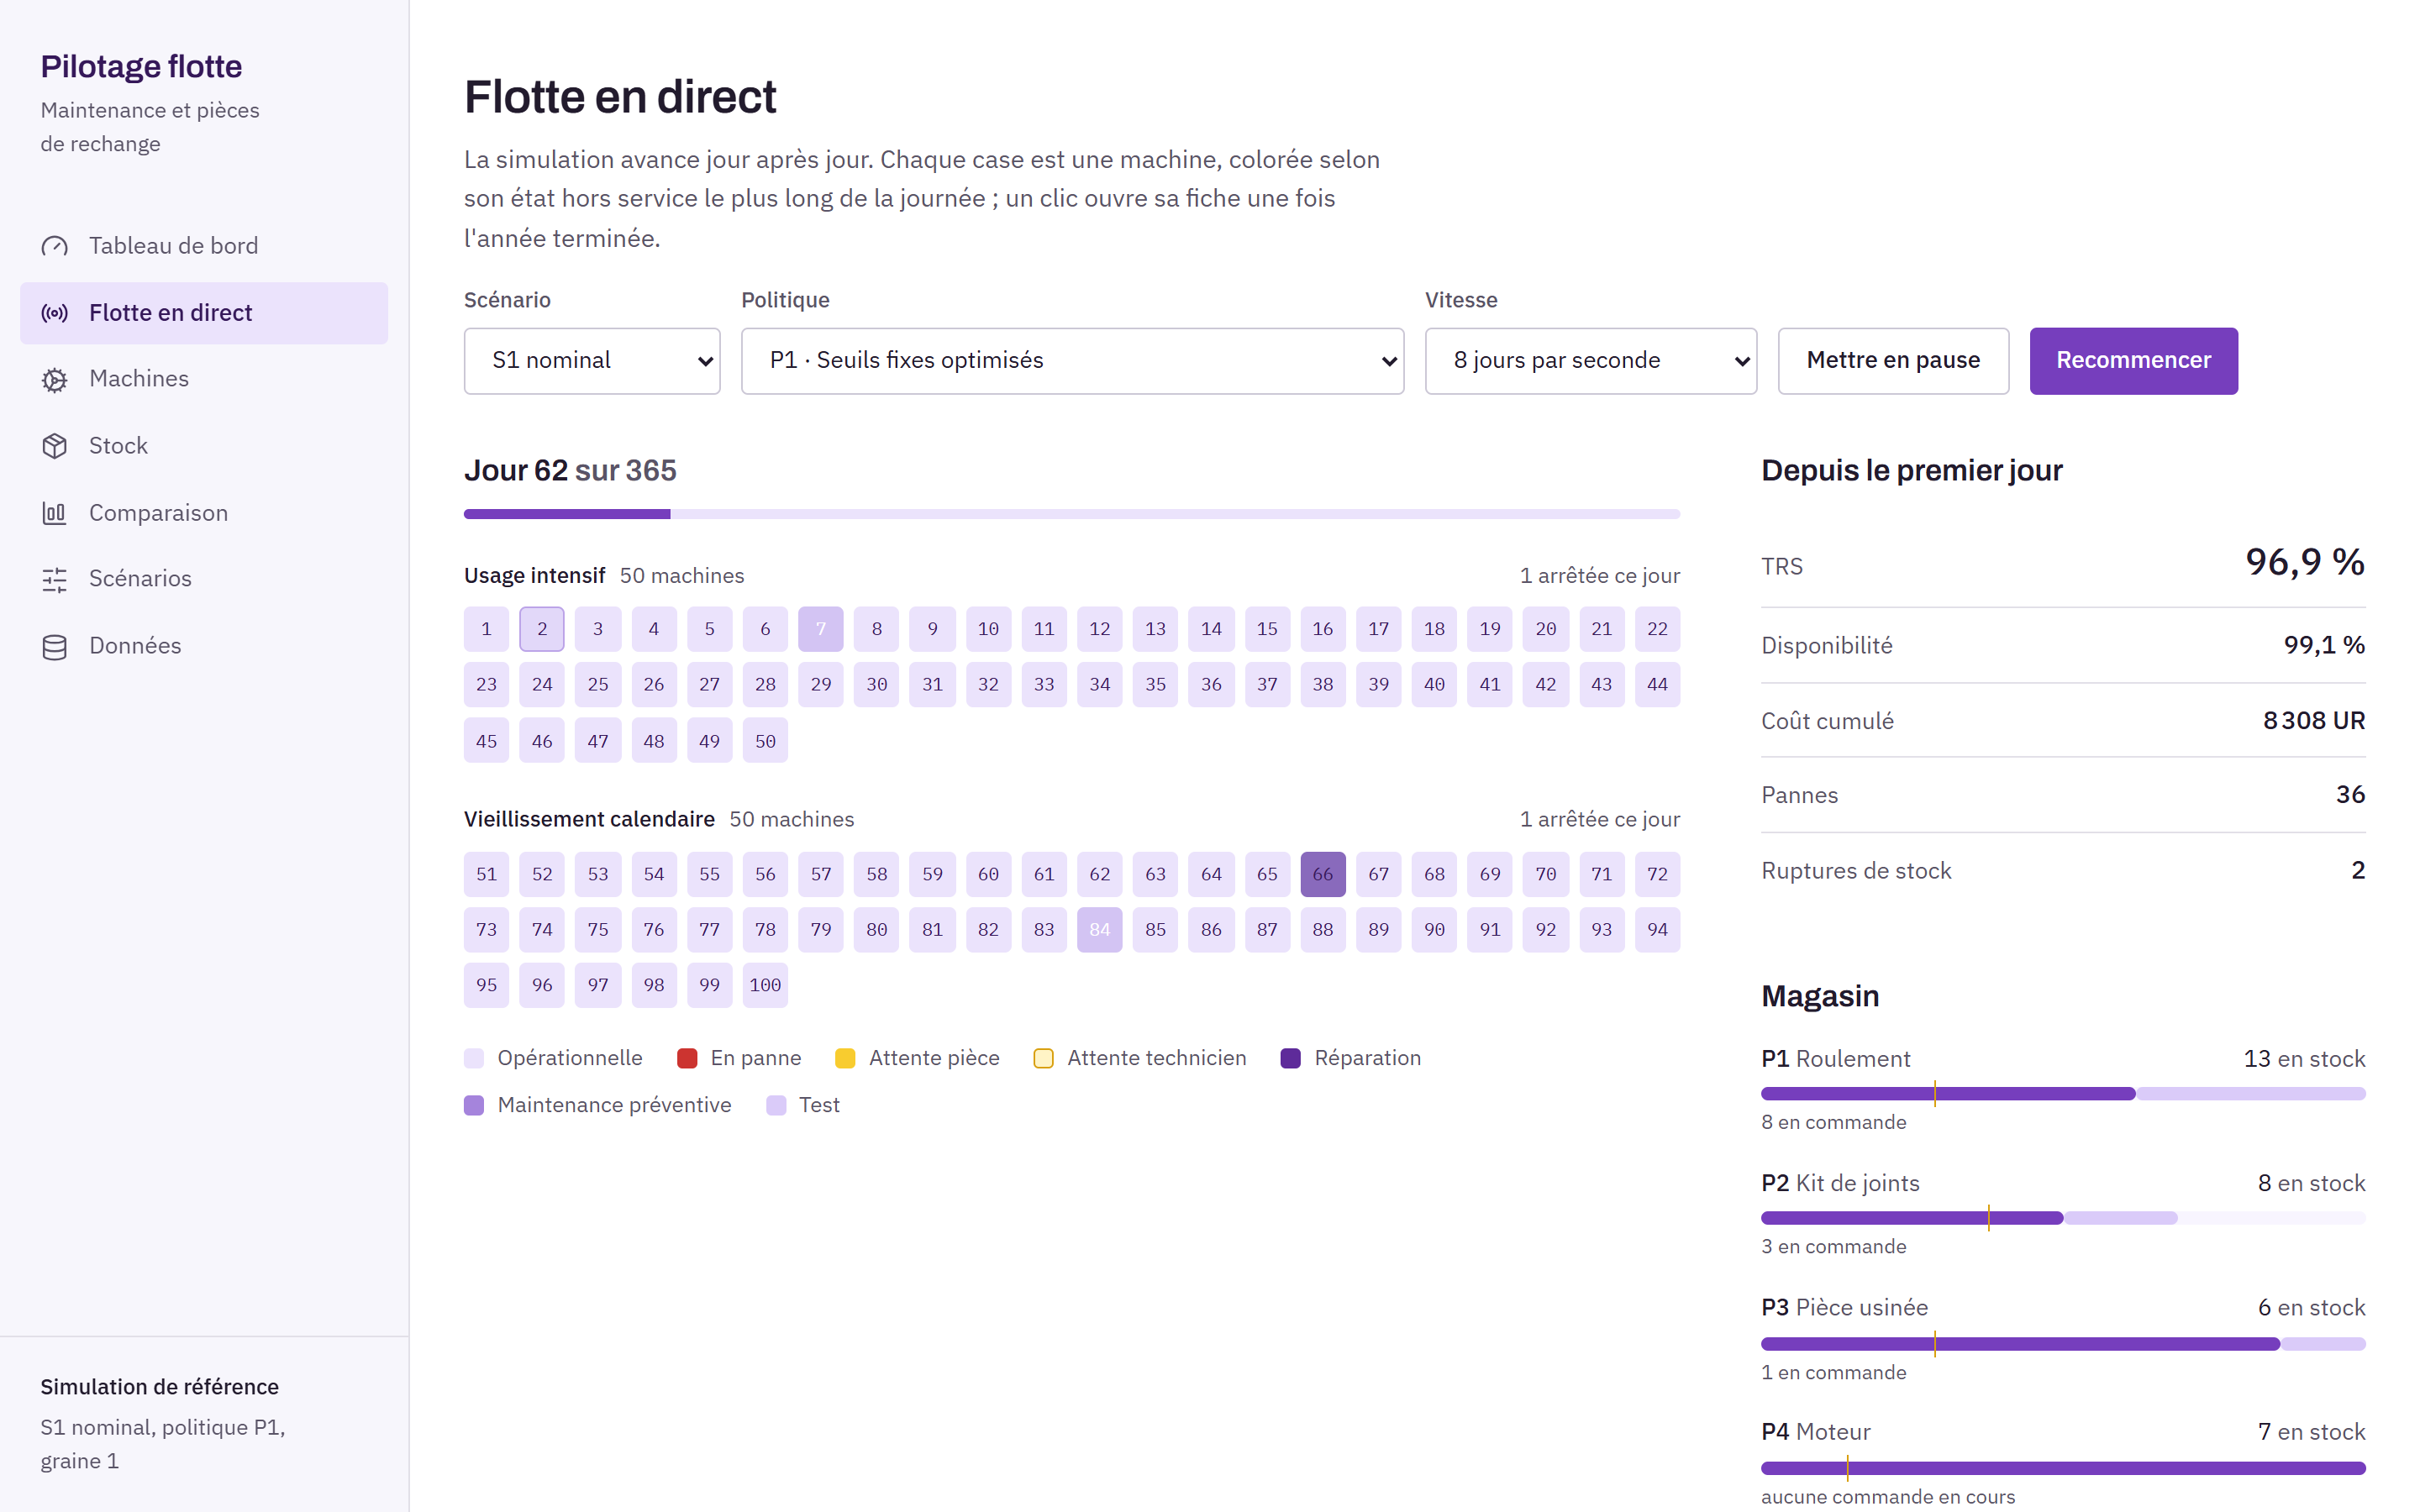
\includegraphics[width=\linewidth]{figures/direct.png}
\caption{Page « Flotte en direct » en cours de simulation.}
\end{figure}

\begin{figure}[H]
\centering
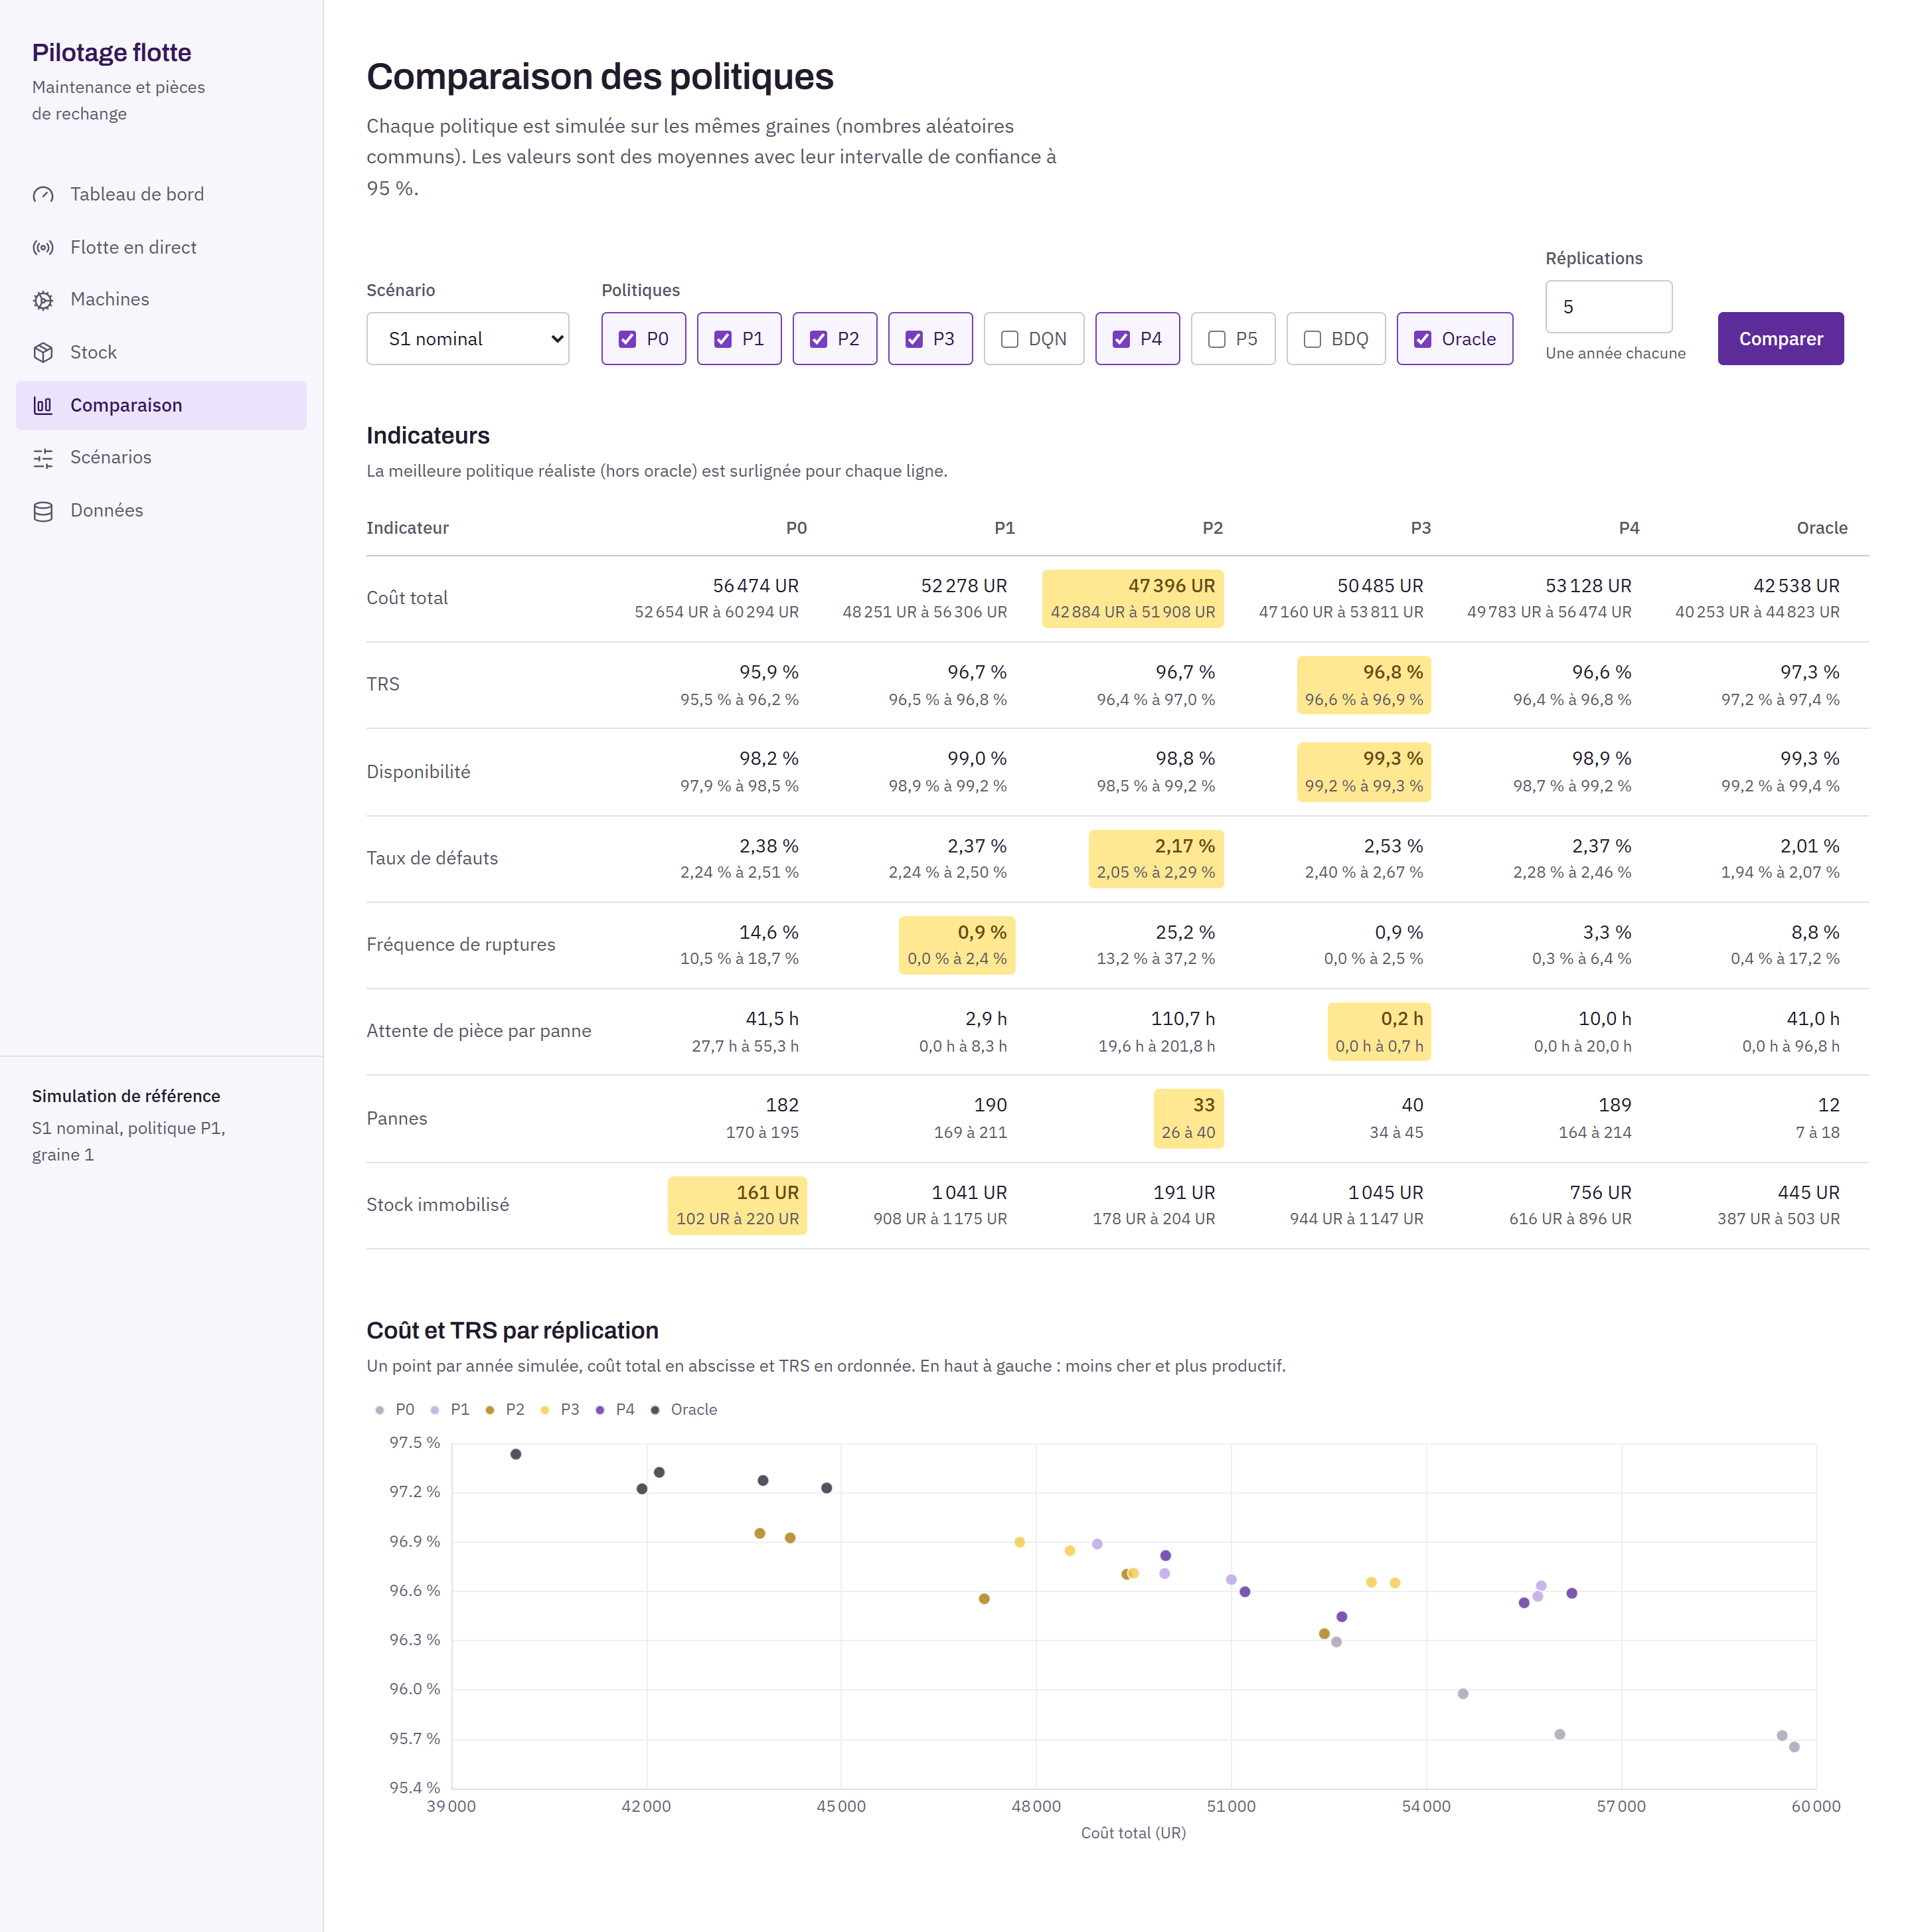
\includegraphics[width=\linewidth]{figures/comparaison.png}
\caption{Page « Comparaison » : indicateurs avec intervalles de confiance et nuage coût, TRS.}
\end{figure}

% ================================================================ 10
\section{Conclusion}\label{sec:conclusion}

\subsection{Bilan}

La question posée par le cahier des charges appelle une réponse nuancée. L'apprentissage profond réduit bien le coût par rapport à une politique à seuils fixes correctement réglée, mais par la prédiction plutôt que par l'apprentissage par renforcement : P3, qui s'appuie sur un réseau de survie, économise 2,1~\% à disponibilité supérieure, et c'est la politique la plus robuste lorsque les délais fournisseurs doublent. Les agents d'apprentissage par renforcement, eux, n'atteignent pas P1 ; le meilleur s'en approche à 1,1~\% près. Une règle de maintenance conditionnelle simple fait mieux que toutes les politiques apprises, avec 9,6~\% d'économie.

Deux enseignements en ressortent. Le premier est que la valeur vient de l'information sur l'état des composants : les politiques qui l'exploitent, P2 et P3, divisent le nombre de pannes par quatre à six, et l'oracle montre qu'il reste encore 10~\% à gagner avec une information parfaite. Le second est que l'apprentissage par renforcement bute ici sur des difficultés concrètes, que le projet a rencontrées et levées une à une : un espace d'actions de plus de $10^{76}$ combinaisons, une récompense bruitée par les pannes de toute la flotte, un critique incapable d'apprendre sans normalisation des récompenses, une politique dont l'action la plus probable diffère de la loi apprise. Chacune est documentée avec sa correction, ce qui vaut autant pour la suite que les chiffres eux-mêmes.

\begin{tabularx}{\linewidth}{@{}l L P{3.2cm}@{}}
\caption{Atteinte des objectifs du cahier des charges}\label{tab:objectifs}\\
\toprule
\hd{Obj.} & \hd{Critère et résultat} & \hd{Verdict} \\
\midrule
O1 & Jeu Azure enrichi (durées, familles, défauts, coûts) ; une fuite d'information temporelle détectée, corrigée et couverte par un test & Atteint \\
O2 & Pannes d'Azure reproduites à 10~\% près : écarts de $-$4,3 à $+$7,9~\% sur 2015, jusqu'à 18~\% sur le seul second semestre & Atteint sur l'année \\
O3 & F1 supérieur à LightGBM : vrai aux deux horizons sur données simulées, à 7 jours seulement sur Azure & Atteint en partie \\
O4 & Coût inférieur à P1 à disponibilité au moins égale : P4 à $+$1,1~\%, P5 à $+$19~\% & Non atteint \\
O5 & $R^2$ supérieur à 0,9 sur des scénarios non vus : de 0,913 à 0,983 & Atteint \\
O6 & Application web de sept pages, parcours principal testé de bout en bout & Atteint \\
\bottomrule
\end{tabularx}

\subsection{Limites}

\begin{itemize}
\item \textbf{Des données réelles elles-mêmes synthétiques.} Le jeu Azure a été généré par Microsoft pour illustrer la maintenance prédictive. Ses pannes sont précédées d'anomalies plus nettes qu'on ne l'observe souvent sur le terrain, ce qui explique en partie le bon score de LightGBM à 24 heures, et sa calibration repose sur une censure informative que nous avons dû corriger par simulation.
\item \textbf{Un simulateur volontairement simplifié.} Les coûts sont exprimés en unités relatives, les fournisseurs n'ont pas de capacité limitée, une pièce déposée n'est jamais réparée ni réutilisée, et les techniciens sont interchangeables.
\item \textbf{Un budget de calcul limité.} Chaque agent a été entraîné avec une seule graine, en quelques centaines de milliers de pas, sur un poste de quatre cœurs, avec des réglages proches des valeurs usuelles. Les écarts entre agents mesurent donc ces entraînements précis plus que les méthodes elles-mêmes ; plusieurs graines d'entraînement, des apprentissages plus longs et un réglage des hyperparamètres seraient nécessaires pour conclure sur les méthodes.
\item \textbf{Un seul scénario d'apprentissage.} Les agents et les seuils sont réglés sur le scénario nominal ; la robustesse est mesurée sans nouvel apprentissage, ce qui correspond à l'usage réel mais pénalise les politiques les plus spécialisées.
\end{itemize}

\subsection{Perspectives}

\begin{itemize}
\item Prolonger l'apprentissage de P5, dont le coût baissait encore à la fin des 200\,000 pas, et donner au BDQ une récompense par machine, qui attribuerait à chaque branche l'effet de sa propre décision.
\item Donner aux agents le risque estimé par le réseau de survie : le codec d'observation le prévoit déjà, et l'agent combinerait alors l'information de P3 et l'adaptation de l'apprentissage par renforcement.
\item Entraîner les agents sur un ensemble de scénarios tirés au hasard (délais, taux de panne, effectifs) plutôt que sur le seul scénario nominal, pour obtenir des politiques robustes par construction.
\item Remplacer la recherche aléatoire de P1 et la grille de P3 par une optimisation bayésienne sur le modèle de substitution, qui évalue un jeu de paramètres en quelques millisecondes.
\item Confronter le simulateur et les modèles à l'historique d'un atelier réel, qui fournirait les durées, les coûts et les pratiques de maintenance que le jeu Azure ne contient pas.
\end{itemize}


% ================================================================ Annexe
\appendix
\section{Reproduire les résultats}\label{sec:reproduire}

Prérequis : Python 3.11 avec uv, Node.js, les cinq fichiers CSV d'Azure dans \texttt{data/raw}.

\begin{tabularx}{\linewidth}{@{}P{7.2cm} L@{}}
\toprule
\hd{Commande} & \hd{Résultat} \\
\midrule
\texttt{uv sync -{}-extra ml} & Installation des dépendances \\
\texttt{uv run pytest} & Tests automatiques \\
\texttt{scripts/calibrate\_azure.py} & Lois de Weibull (tableau~\ref{tab:weibull}) \\
\texttt{scripts/validate\_azure.py} & Validation O2 (tableau~\ref{tab:validation}) \\
\texttt{scripts/optimize\_p1.py} & Seuils de P1 \\
\texttt{scripts/train\_predictor.py} & Tableau~\ref{tab:pred-sim} ; avec \texttt{-{}-source azure}, tableau~\ref{tab:pred-azure} \\
\texttt{scripts/tune\_p3.py} & Seuils de P3 \\
\texttt{scripts/train\_rl.py -{}-level n1} & Agent P4 ; \texttt{-{}-level n2} pour P5 \\
\texttt{scripts/train\_bdq.py} & Branching Dueling Q-Network \\
\texttt{scripts/train\_rl.py -{}-level reduced -{}-algo dqn} & DQN du niveau réduit \\
\texttt{scripts/choose\_agent\_mode.py} & Mode de jeu de P4 et P5 \\
\texttt{scripts/train\_surrogate.py} & Modèle de substitution \\
\texttt{scripts/sensitivity.py} & Indices de Sobol (figure~\ref{fig:sobol}) \\
\texttt{scripts/evaluate\_policies.py -{}-robustness} & Évaluation finale (section~\ref{sec:evaluation}) \\
\texttt{scripts/export\_report\_data.py} & Données des graphiques de ce rapport \\
\bottomrule
\end{tabularx}

% ================================================================ Références
\begin{thebibliography}{99}
\addcontentsline{toc}{section}{Références}
\small
\NoAutoSpacing
\setlength{\itemsep}{0.15em}
\bibitem{azure} Microsoft Azure Predictive Maintenance, jeu de données publié sur Kaggle, \url{https://www.kaggle.com/datasets/arnabbiswas1/microsoft-azure-predictive-maintenance}.
\bibitem{gensheimer} M. F. Gensheimer et B. Narasimhan, «~A scalable discrete-time survival model for neural networks~», \emph{PeerJ}, 7:e6257, 2019.
\bibitem{dqn} V. Mnih et al., «~Human-level control through deep reinforcement learning~», \emph{Nature}, 518, p.~529-533, 2015.
\bibitem{ppo} J. Schulman et al., «~Proximal policy optimization algorithms~», arXiv:1707.06347, 2017.
\bibitem{masking} S. Huang et S. Ontañón, «~A closer look at invalid action masking in policy gradient algorithms~», \emph{FLAIRS}, 2022.
\bibitem{bdq} A. Tavakoli, F. Pardo et P. Kormushev, «~Action branching architectures for deep reinforcement learning~», \emph{AAAI}, 2018.
\bibitem{ensembles} B. Lakshminarayanan, A. Pritzel et C. Blundell, «~Simple and scalable predictive uncertainty estimation using deep ensembles~», \emph{NeurIPS}, 2017.
\bibitem{saltelli} A. Saltelli et al., \emph{Global Sensitivity Analysis: The Primer}, Wiley, 2008.
\bibitem{sb3} A. Raffin et al., «~Stable-Baselines3: Reliable reinforcement learning implementations~», \emph{Journal of Machine Learning Research}, 22(268), 2021.
\bibitem{impeccable} Impeccable, catalogue d'anti-modèles d'interface, \url{https://impeccable.style}.
\end{thebibliography}

\end{document}
